% 1. Develop, test and deploy a new software workflow to incorporate external packages into Bonsai's C# environment.

% 2. Incorporate a suite of machine-learning-driven analysis tools into the Bonsai environment to implement:
% 2a. video-based  behavioural analysis
% 2b. real-time interfacing of population-scale activity with laboratory control  
% 2c. evaluate competing data analytic approaches within a single experimental framework

\section{Details of the proposed resource enhancements}

While Bonsai 



We
propose to create software infrastructure to enable the\textbf{ integration of advanced data analysis methods} into
Bonsai (Section~\ref{sec:infrastructure}).
%
To demonstrate the use of this infrastructure, and to provide Bonsai users with
an initial set of advanced machine intelligence neural data analysis methods,
we will add to the Bonsai ecosystem machine learning functionality to control
neuroscience experiments and to analyse data generated by them
(Section~\ref{sec:functionality}).

This initial set of methods should demonstrate to Bonsai users, and to
machine-learning methods developers, the potential of embedding
machine-learning functionality into the experimental control loop. We propose
user engagement activities to expose both of these groups to this
potential (Section~\ref{sec:userEngagement}).  As data-analysis method
developers recognise this opportunity, they will become interested in
contributing their methods to the Bonsai ecosystem, ensuring the
\textbf{long-term sustainability} of the proposed resource.

Adding machine learning functionality to the experimental control loop will
make possible the implementation of experiments with unprecedented levels of
control. Moreover, equipping experimental scientists without programming
experience with machine learning tools will considerably increase the
application of machine learning to the biosciences, which most probably will
translate into groundbreaking scientific discoveries.


Currently Bonsai has its own package manager, and its community of users have
already extended Bonsai's functionality with several contributed packages.
%
However, these packages need to
be written in C\#, while most current neuroscience data analysis methods are
written in Python, R or Matlab. We propose to add to Bonsai capabilities to
communicate with software written in these languages
(Section~\ref{sec:softwareInfrastructure}).  These capabilities will allow a
large number of neuroscience data analysis methods to be easily integrated into
the Bonsai ecosystem and will provide Bonsai users a large repertoire of
advanced machine learning methods for their behavioural and neural data
analysis.
%
Using these capabilities we will integrate into Bonsai an initial set of
state-of-the art behavioural and neural data analysis methods
(Section~\ref{sec:functionality}).

Developers of advanced data-analysis methods should become interested in
integrating them into the Bonsai ecosystem, as it will allow their methods to
reach the wide Bonsai user community. In addition this integration will enable
method developers to easily compare the performance of their methods with
that of many methods previously integrated into the Bonsai ecosystem. Method
developers will thus become a new type of Bonsai users, which will contribute
to the \textbf{sustainability} of the proposed resource beyond the period of
BBSRC-BBR funding.

% Scientific advances rely on \textbf{reproducibility}, which in turn depends on standardized tools for experimental control and analysis, shared between laboratories (Baker, 2016; Ioannidis, 2005). Although such tools exist in genetics, astronomy, physics and medicine (Fish et al., 2016; Abdalla et al., 2018, CERN Education, Communications and Outreach Group, 2018, Dickinson et al., 2016, Bycroft et al., 2018), they are mostly lacking in neuroscience, which in itself suffers from a paucity of reproducible discoveries (Baker, 2016; Botvinik-Nezer et al., 2020; Button et al., 2013). Bonsai is an excellent tool for reproducible data acquisition and experimental control. For example, an experiment implemented in Bonsai can be replicated in
% any laboratory by just sharing a Bonsai configuration file. With the addition of the proposed machine learning functionality Bonsai will extend this
% reproducibility to the domain of data analysis
% (Section~\ref{sec:reproducibility}).

\begin{figure}
  
\includegraphics[width=4in]{figures/proposed_bonsai_extensions.png}
  \caption{Proposed extensions to Bonsai}
  \label{fig:proposedBonsaiExtensions}
\end{figure}


\subsection{Software infrastructure}
\label{sec:infrastructure}

\begin{comment}
Bonsai does not currently provide machine learning functionality. For instance,
the close-loop experimental control depicted in
Figure~\ref{fig:bci} cannot be currently implemented in
Bonsai. It represents the control of an experiment where a subject guides the
mouse position in a computer screen with her brain activity (Section~\ref{}).
Nodes highlighted in colour require machine intelligence functionality currently
not available in Bonsai.
%
\end{comment}

We propose to create software infrastructure to add machine intelligence
functionality to the Bonsai ecosystem in general
(Section~\ref{sec:generality}) and extensible ways
(Section~\ref{sec:extensibility}).

\subsubsection{Generality}
\label{sec:generality}

The number of current machine learning algorithms is very large and it is
continuously increasing. We intend to build a small number of machine
intelligence operators in Bonsai (Section~\ref{sec:bonsai},
Figure~\ref{fig:bonsai}c) that can be configured to provide the functionality
of all machine learning algorithms.

For this, we will build on abstractions used in the \texttt{scikit-learn}
library. The success of this library is, to a large extent, due to its simple
and general application programming interface \citep[API;][]{buitinckEtAl13}.
%
This API consists of three complementary interfaces: an \texttt{Estimator}
interface for building and fitting models, a \texttt{Predictor} interface for
making predictions and a \texttt{Transformer} interface for converting data.
%
Using only these three interfaces \texttt{scikit-learn} provides
implementations of a large number of machine learning algorithms for
dimensionality reduction, clustering, classification and regression.

Inspired by \texttt{scikit-learn}, Bonsai will have three types of operators:
\texttt{Estimators}, \texttt{Predictors} and \texttt{Transformers}. Each of
these operators will be instantiated by objects implementing the corresponding
interface.
%
As an example, consider the close-loop system for the control of a computer
cursor with neural activity represented in Figure~\ref{fig:bci}a. The Bonsai
graphical program for this system is given in Figure~\ref{fig:bci}b. The
objects instantiating the SpikeThresholdDetector, the KiloSortSpikeSorter and
GPFAlatentsExtractor will implement the \texttt{Transformer} interface (blue),
and the object instantiating the TimeSeriesForestClassifier will implement the
\texttt{Predictor} interface (green; Figure~\ref{fig:bci}b, top).
%
The parameters for the SpikeThresholdDetector and the KiloSortSpikeSorter will
be set manually by the user, as is commonly done in practice. The parameters of
the GPFAlatentsExtractor will be learnt offline in an unsupervised way by an
\texttt{Estimator} (red) in a second pipeline (Figure~\ref{fig:bci}b, middle).
Finally, the parameters of the TimeSeriesForestClassifier will also be learnt
offline, but in a supervised way, by another \texttt{Estimator} in a third
pipeline (Figure~\ref{fig:bci}b, bottom).

\begin{figure}
   \begin{center}
       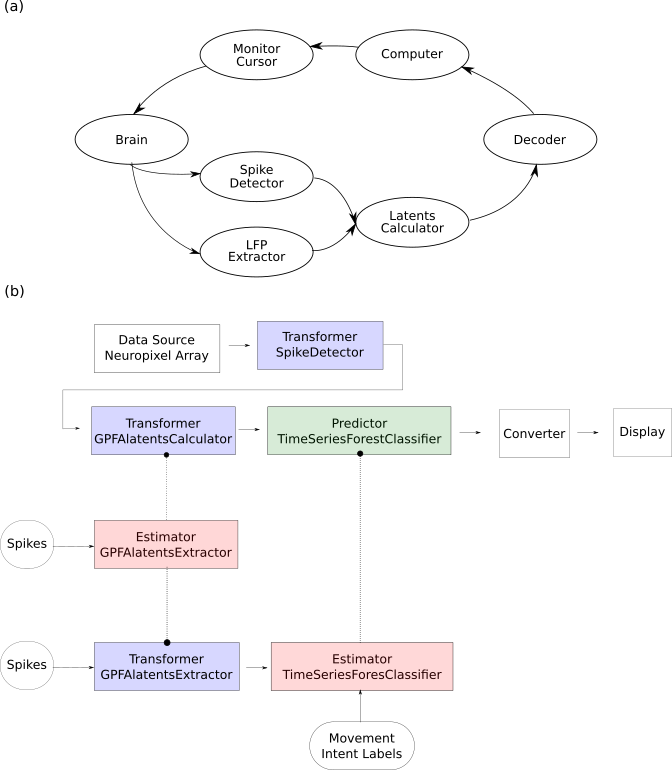
\includegraphics[width=4in]{figures/bci.png}
       \caption{Close-loop system for controlling a computer cursor with brain activity}
     \label{fig:bci}
   \end{center}
\end{figure}

\begin{comment}
    The spike detector transforms membrane
potentials into spike sequences. The spike sorter transforms spikes sequences
into lists of spikes, one list per neuron. The latents extractor transforms
multi-neuron lists of spikes into latent trajectories summarising the
multi-neuron spiking activity.  The neural decoder predicts the next cursor
position from the latent trajectories.
\end{comment}

\begin{comment}
middle, whose output will set
As in this library,
there will be three type of machine intelligence operators in Bonsai:
%
estimator operators for building and fitting models, predictor operators for
making predictions and transformer operators for converting data. These
operators will be implemented by objects exposing the corresponding interfaces.

The estimator interface exposes a fit method for learning a model from training
data.  This method is called with training data (e.g., supplied as two arrays
X\_train and y\_train in supervised learning estimators). Its task is to run a
learning algorithm and to determine model-specific parameters from the training
data.  All supervised and unsupervised learning algorithms (e.g., for
classification, regression or clustering) will be offered as objects
implementing this interface. Machine learning tasks like feature extraction,
feature selection or dimensionality reduction will also be provided as
estimators.

The predictor interface extends the notion of an estimator by adding a predict
method that takes an array X\_test and produces predictions for X\_test, based
on the learned parameters of the estimator (we call the input to predict
“X\_test” in order to emphasise that predict generalises to new data). In the
case of supervised learning estimators, this method typically returns the
predicted labels or values computed by the model.

Since it is common to modify or filter data before feeding it to a learning
algorithm, the transformer interface defines a transform method. It takes as
input some new data X\_test and yields as output a transformed version of
X\_test. Preprocessing, feature selection, feature extraction and
dimensionality reduction algorithms will be provided as transformers in Bonsai.

Bonsai will provide the ability to compose new
estimators from several base estimators. Composition mechanisms can be used
to combine typical machine learning workflows into a single object which is
itself an estimator, and can be employed wherever usual estimators can be used.
Composition of estimators will be done with Pipeline objects that chain multiple estimators into a single one. This is useful
since a machine learning workflow typically involves a fixed sequence of processing steps (e.g., feature extraction, dimensionality reduction, learning and making
predictions), many of which perform some kind of learning. A sequence of N such
steps can be combined into a Pipeline if the first N-1 steps are transformers;
the last can be either a predictor, a transformer or both.

\end{comment}

\subsubsection{Extensibility}
\label{sec:extensibility}

To incorporate machine learning functionality into the Bonsai ecosystem, we
could
implement this functionality directly into Bonsai, as done in
\texttt{scikit-learn}. Alternatively, or in addition, we could build software
infrastructure to facilitate the integration of existing machine learning
software into Bonsai. We chose to begin with the second alternative because
high-quality implementations of machine learning functionality already exist,
which can be quickly integrated into the Bonsai ecosystem. In addition, the
second alternative is more sustainable, as it will allow the continued addition
of new machine learning functionality to Bonsai after the completion of the
BBSRC-BBR funding period. Later we may decide to implement some widely-used
machine learning functionality directly into Bonsai (e.g., for performance or
robustness issues).

Currently Bonsai has its own package manager, and its community of users have
already extended Bonsai's functionality with several contributed packages
(e.g., \ldots). However, these packages need to be written in C\#, while most
current data analysis methods are written in Python, R or Matlab. We propose to
add to Bonsai capabilities to communicate with software written in these
languages.

Fortunately, there exist software that allow C\# program
to call and be called by programs in these other languages. For the
communication of C\# programs with Python we will use
Python.NET\footnote{\href{https://github.com/pythonnet/pythonnet}{https://github.com/pythonnet/pythonnet}},
with R programs we will use
R.Net\footnote{\href{https://github.com/rdotnet/rdotnet}{https://github.com/rdotnet/rdotnet}}
and with Matlab we will use the built in Matlab .NET
interface\footnote{\href{https://uk.mathworks.com/help/matlab/matlab\_external/using-net-from-matlab-an-overview.html}{https://uk.mathworks.com/help/matlab/matlab\_external/using-net-from-matlab-an-overview.html}}.
In cases where these software cannot support some type of communication between
C\# and another language we will use the messaging library
ZeroMQ\footnote{\href{https://zeromq.org/}{https://zeromq.org/}}.

Using the previous software, we will build C\# wrappers around machine
intelligence programs written in other languages, so that these programs
implement the \texttt{Estimator}, \texttt{Predictor} or \texttt{Transformer}
interfaces and can be integrated into Bonsai as machine intelligence operators.

\subsection{Machine intelligence functionality to be added to Bonsai}
\label{sec:functionality}

We propose to initially add to Bonsai machine intelligence functionality to
support neuroscience experiments because, currently, neuroscience is the
research area with the largest number of Bonsai users. Within neuroscience, we
propose to add functionality for video-based behavioural analysis
(Section~\ref{sec:videoBasedBehavioralAnalysis}) and for running
brain-computer-interface (BCI) experiments (Section~\ref{sec:bci}), since these tasks
are relevant to many Bonsai users, and recent advances in machine learning
will greatly improve their implementation in Bonsai.

\subsubsection{Video-based behavioral analysis}
\label{sec:videoBasedBehavioralAnalysis}

Precisely quantifying animal behaviour is an essential step toward understanding
brain function.  Deeplabcut is a Python-based software for tracking animal body
parts \citep{mathisEtAl18}, which it is currently well integrated with
Bonsai~\citep{kaneEtAl20}. Here we propose extensions to Bonsai to extract
other informative features from video recordings.

\begin{description}

    \item[Motion sequencing]\citep[MoSeq;][]{wiltschkoEtAl15}: extracts patterns
        of behaviour that repeat over time (i.e., syllables of behaviour) from
        video data. For instance, it parses (in an unsupervised way) the
        behaviour of a mouse in an arena into segments of time where a mouse
        was running, rearing and grooming. It uses a hidden Markov model and it
        is implemented in Python\footnote{Code for MoSeq can be requested from
        the Datta laboratory, as indicated at
        \href{http://datta.hms.harvard.edu/research/behavioral-analysis/}{http://datta.hms.harvard.edu/research/behavioral-analysis/}.}.
        After trained MoSeq can be used to detect behavioral syllables online.

    \item[Decoding behaviour from neural
        activity]\citep[BehaveNet;][]{battyEtAl19} combines hidden Markov
        models with convolutional autoencoders and discriminative models to
        decode video data from neural recordings. It is implemented in
        Python\footnote{\href{https://github.com/themattinthehatt/behavenet}{https://github.com/themattinthehatt/behavenet}}.
        After trained it can be used online to decode video data and detect
        behavioral syllables.

    \item[Interpretable latents for behavioral videos]\citep[Partitioned
        Subspace Variational Autoencoder, PS-VAE;][]{whitewayEtAl21}: produces
        interpretable low-dimensional representations of behavioral videos by
        combining the output of pose-estimation algorithms (e.g., DeepLabCut)
        with unsupervised dimensionality reduction methods. These
        low-dimensional representations facilitate downstream behavioral and
        neural analyses. It is based on autoencoders and is implemented in
        Python\footnote{code for PS-VAE is embedded in the BehaveNet code
        \href{https://github.com/themattinthehatt/behavenet}{https://github.com/themattinthehatt/behavenet}.
        Please refer to class \texttt{PSVAE} in 
        \texttt{behavenet.models.vaes.py}.}. After trained it can be used
        online to extract low-dimensional features and perform downstream
        processing.

\end{description}

\subsubsection{Brain-computer-interface applications}
\label{sec:bci}

We propose to add functionality into Bonsai for the implementation of
brain-computer-interface (BCI) applications illustrated in Figure~\ref{fig:bci}. In
this implementation voltage recordings from the brain will be converted into
spikes fired by single neurons by a \texttt{SpikeDetector}
(Section~\ref{sec:spikeDetection}), or to local field potentials (LFP) by an
\texttt{LFPextractor} (Section~\ref{sec:lfpExtraction}). Next, neural activity
(spikes or LFPs) will be represented in a low-dimensional latent space by a
\texttt{LatentsCalculator}. Finally, a \texttt{Decoder} will extract the
intended behavior of the animal from this low-dimensional representation.

\paragraph{Spike detection}
\label{sec:spikeDetection}

Spikes from multiple neurons can be detected in recordings from a single
electrode inserted in neural tissue. Spike sorting is the computational step
used to assign each spike to the neuron that generated it. Most spike sorting
algorithms are designed to work offline (i.e., to use a complete recording
session, after this session terminated). Online spike sorting (i.e., the task
of assigning spikes to individual neurons as recordings are being aquired) is a
still unsolved task, specially for recording devices with large number of
electrodes.
%
However, for the type of BCI application proposed here, previous studies have
shown that spike sorting is not beneficial and high performance can be retained
by just detecting spikes, without assigning them to invidivual
neurons~\citep{trautmannEtAl19,todorovaEtAl14}. Thus, for the BCI application
proposed here we will only detect spikes with a simple zero-corssing method,
and not assign them to individual neurons.  We will, however, integrate into
Bonsai two offline spike sorting methods, Kilosort~\citep[][written in Matlab]{pachitariuEtAl16} and MountainSort~\citep[][written in
Python]{chungEtAl17}, to provide Bonsai users spike sorting functionality for
applications that benefit from it.

\paragraph{LFP extraction}
\label{sec:lfpExtractor}

Spikes are extracted from a higher-frequency range of extracellularly recorded
voltages. Local field potentials (LFPs) 
are another important signal to understand brain function, which is extracted
from a lower-frequency range of these voltages. We propose to use in-house
functions implemented in Python to compute LFPs.

\paragraph{Low-dimensional representations of neural recordings}
\label{sec:lowDimensionalRepresentation}

Bonsai is well integrated with OpenEphys~\citep{siegleEtAl17}, which allows
scientists to record neural data from a large number of devices. However, it
lacks functionality to process these recordings. Here we describe software that
we propose to integrate into Bonsai to extract interpretable summary statistics
(i.e., latent variables) from neural spiking activity.

\begin{description}

    \item[Gaussian Linear Dynamical
        System]\citep[GLDS;][]{andersonAndMoore12}: with sufficiently large
        bin sizes, spike counts can be modelled as Gaussian random processes.
        This Gaussianity assumption greatly simplifies the estimation of
        parameters of linear dynamical system (LDS) models, as well as
        inferences about their states. After models parameters have been
        learned, GLDS can be used online. A unique feature of GLDS is that the
        posterior distribution of states given all observation up to the
        present can be calculated efficiently. This estimate of the posterior
        distribution can be used online for experimental control, as we
        propose in Section~\ref{sec:comparisonOfMultipleMethods}. We will use an R implementation of GLDS
        which allows the use of external
        inputs\footnote{\href{https://github.com/joacorapela/kalmanFilter}{https://github.com/joacorapela/kalmanFilter}}.

    \item[Poisson Linear Dynamical System]\citep[PLDS;][]{mackeEtAl15}: for
        smaller bin sizes, spike counts are better modelled as Poisson random
        processes, rather than Gaussian ones. The algorithm described in
        \citet{mackeEtAl15} can estimate the parameters of a LDS, and make
        inferences about its states, from Poisson distributed observations.  We
        propose to interface Bonsai with a Matlab implementation of
        PLDS\footnote{\href{https://bitbucket.org/mackelab/pop\_spike\_dyn/src/master/}{https://bitbucket.org/mackelab/pop\_spike\_dyn/src/master/}}
        that uses variational inference. PLDS does not provide online estimates
        of the states, since data from a full trial is needed for state
        inference.

    \item[Hidden Markov Model]\citep[HMM;][]{rabiner89}: as LDSs, HMMs model a
        time series of observations as random processes conditioned on hidden
        states. However, in HMMs hidden states are discrete random variables,
        while in LDSs they are continuous ones. In some application domains
        (e.g., speech, epilepsy) discrete state assumptions are more pertinent
        than continuous ones. We propose to use an R implementation of
        HMMs\footnote{\href{https://github.com/joacorapela/hiddenMarkovModels}{https://github.com/joacorapela/hiddenMarkovModels}}.
        As GLDSs, once trained, HMMs can be used online to infer the posterior
        distribution of states given observations.

    \item[Gaussian Processes Factor Analysis]\citep[GPFA;][]{yuEtAl09}: as
        LDSs, GFPA models represent a time series of observation as random
        processes conditioned on hidden states. However, in GPFA models the
        state dynamics are nonlinear, while in LDS models they are linear.
        Thus, GPFA models are more general than LDS ones. As GLDS models, GPFA
        models assume that observations conditioned on states are Gaussian
        random processes. We propose to use a Matlab implementation of
        GPFA\footnote{\href{https://users.ece.cmu.edu/~byronyu/software/gpfa0203.tgz}{https://users.ece.cmu.edu/~byronyu/software/gpfa0203.tgz}}.
        GPFA models do not provide online estimates of the states, since data
        from the full trial are needed for state estimates.

    \item[Sparse Variational Gaussian Processes Factor
        Analysis]\citep[svGPFA;][]{dunckerAndSahani18}: is similar to GPFA, but
        models point process observations (i.e., single spikes as opposed to
        spike counts). We propose to use a Python implementation of
        svGPFA\footnote{\href{https://github.com/joacorapela/svGPFA}{https://github.com/joacorapela/svGPFA}}.
        svGPFA models do not provide online estimates of states, since data
        from the full trial are needed for state estimates.

    \item[Latent factor analysis through dynamical
        systems]\citep[LFADS;][]{pandarinathEtAl18}: uses an autoencoder
        framework, with recursive neural networks, to infer continuous states
        conditioned on spike counts, similar to those inferred by GPFA. We
        propose to use a Python implementation at
        LFADS\footnote{\href{https://github.com/tensorflow/models/tree/master/research/lfads}{https://github.com/tensorflow/models/tree/master/research/lfads}.}.
        As GPFA, LFADS do not provide online estimates of states.

\end{description}

\paragraph{Low-dimensional representations of local-field potentials}
\label{sec:lowDimensionalRepresentationsOfLFPs}

Spikes are extracted from a higher-frequency range of extracellularly recorded
voltages. Local field potentials (LFPs) are computed from a lower-frequency
range and are another important signal to understand brain function. We propose
to use states inferred from LFPs by GLDS, GPFA, HMM and LFADS
(Section~\ref{sec:lowDimensionalRepresentation}) as
low-dimensional representations of the LFP.

\paragraph{Neural decoding}
\label{sec:neuralDecoding}

In order to use low-dimensional representations of spiking activity and/or of
LFPs to guide the control of experiments, we need a decoder to optimally map
these low-dimensional representations to experimental controls.
%
We propose to implement in Bonsai several decoding/classification algorithms:
k-nearest neighbour, linear discriminative analysis, support vector machines,
random forests, artificial neural networks, naive Bayes and Gaussian process
classifiers.

\paragraph{Comparing multiple data-analysis methods}
\label{sec:comparisonOfMultipleMethods}

% We propose to add functionality to Bonsai to facilitate multi-method
% comparisons in user-supplied datasets.

Below we describe a comparison that we
will perform in Bonsai to asses the relative performance of the methods
described in the previous sections, using neural recordings from behaving rats.
These recordings are currently being performed, to address scientific questions,
at the laboratory of Prof.~Akrami in the SWC.
%
Details of the experimental task appear in~\citet{akramiEtAl18}.
%
Briefly, in this task there are three nose ports (left, centre, right). Rats
initiate a trial by inserting their nose in the centre port for the duration of
the fixation period, until they hear a Go stimulus. During the fixation period
two stimuli $s_a$ and $s_b$ are presented. Rats should decide which stimuli is
louder. If $s_a$ is louder than $s_b$ the correct action is to poke the nose
into the right port in order to collect a liquid reward, and if $s_b$ is louder
than $s_a$ the correct choice is the left port.

We will use high-density Neuropixel spike and LFP recordings from the rats
performing this task to learn low-dimensional representations of spiking
activity and LFPs during the decision time period (between the presentation of
the last auditory stimuli and the presentation of the Go stimulus), using the
methods described in
Sections~\ref{sec:lowDimensionalRepresentation}
and~\ref{sec:lowDimensionalRepresentationsOfLFPs}. We will also learn the
parameters of the classifiers described in Section~\ref{sec:neuralDecoding} to
optimally classify animal decisions (poke the nose into the right/left port)
based on the previous low-dimensional representations.

We will compare the decoding accuracy of all decoders. This comparison will
tells us, for the auditory working memory task, which neural data type (spikes
or LFPs), which low-dimensional representation method (e.g., LDS or Gaussian
processes), and which decoder (e.g., Bayesian or ANN) yields the best decodings
in state-of-the-art neural recordings from behaving animals.

\begin{comment}

\subsection{Interfacing Bonsai with Python, R and Matlab data analysis software}
\label{sec:bonsaiPythonMatlabCommunication}

Bonsai is written in C\# and most neural data-analysis methods are written in
Python, R or Matlab. Fortunately, there exist software that allow C\# program
to call and be called by programs in these other languages. For the
communication of C\# programs with Python we will use
Python.NET\footnote{\href{https://github.com/pythonnet/pythonnet}{https://github.com/pythonnet/pythonnet}},
with R programs we will use
R.Net\footnote{\href{https://github.com/rdotnet/rdotnet}{https://github.com/rdotnet/rdotnet}}
and with Matlab we will use the built in Matlab .NET
interface\footnote{\href{https://uk.mathworks.com/help/matlab/matlab\_external/using-net-from-matlab-an-overview.html}{https://uk.mathworks.com/help/matlab/matlab\_external/using-net-from-matlab-an-overview.html}}.
In cases where these software cannot support some type of communication between
C\# and another language we will use the messaging library
ZeroMQ\footnote{\href{https://zeromq.org/}{https://zeromq.org/}}.

\end{comment}

\subsection{Testing with neuroscience data}
\label{sec:testingWithNeuroscienceData}

Multiple groups at the SWC currently use Bonsai for data acquisition and
experimental control. Carefully testing the functionality of new software is
essential to ensure its correct functionality. We propose to use the SWC large
internal Bonsai user base to test the functionality we will add to Bonsai,
before distributing it to the general public.

\subsection{Reproducibility with Bonsai}
\label{sec:reproducibility}

The current version of Bonsai facilitates reproducibility of data acquisition
and experimental control across laboratories. Most data acquisition and
experimental control aspects of an experiment can be reproduced across
different laboratories by sharing a Bonsai configuration file.
%
By adding data analysis functionality to Bonsai, besides reproducing my data
acquisition and experimental control, Bonsai users will also be able to reproduce
data analysis functionality.

We will demonstrate each machine intelligence functionality added to Bonsai
(Section~\ref{sec:functionality}) and the multiple
data-analysis methods comparisons
(Section~\ref{sec:comparisonOfMultipleMethods}) in Bonsai experiments. We will
then distribute Bonsai configuration files for users to reproduce these
demonstrations.

\subsection{Measurable targets}
\label{sec:measurableTargets}

We propose to assess the progress of the proposed project using three different
types of targets.
%
First, we will have targets associated with each release to the general public
of the software components described in Sections~\ref{sec:infrastructure}
and~\ref{sec:functionality}.
%
Second, we will monitor user activity in the Bonsai
forum\footnote{\href{https://groups.google.com/g/bonsai-users}{https://groups.google.com/g/bonsai-users}},
and publications citing Bonsai that use th new machine larning functionality,
to estimate the number of Bonsai users using this functionality.
%
Third, we will count the number of machine learning methods that are integrated
into the Bonsai ecosystem by us and by other method developers.

\begin{comment}

\begin{description}

    \item[implementation of software infrastructure]
        (Section~\ref{sec:infrastructure}) includes the
        implementation of the machine abstractions, described in
        Section~\ref{},
        and of the capabilities to allow Bonsai communicate with
        software written in other languages, described in Section~\ref{}. We
        will consider this target completed when we can implement a simple BCI
        application, with the architecture depicted in Figure~\ref{}, with
        machine learning functionality provided by software in Python, Matlab
        and R.

    \item[implementation of functionality] (Sections~\ref{sec:functionality})
        includes the integration into Bonsai of machine learning software for
        video-based behavioral analysis (Section~\ref{}) and for
        BCI applications (Section~\ref{}). Completion of
        this target requires that Bonsai can perform each of these tasks
        separately, in conjunction with software written in Python, R and
        Matlab.

    \item[internal testing] multiple groups at the SWC use Bonsai to control
        their experiments. 

        Bonsai Github repository and the success use by Bonsai users

    \item Bonsai users use the implemented machine learning functionality. We
        propose to evaluate this target by checking in the Bonsai user forum
        the frequency with which a novel machine learning functionality is
        discussed, and by tracking publications using this functionality.

    \item method developers integrate their methods into the Bonsai ecosystem.
        The integration of machine learning functionality into Bonsai will use
        Bonsai's package manager. We propose to use this package manager to tack
        the number of machine intelligence methods integrated into Bonsai.

\end{description}

\end{comment}

\begin{comment}

\subsection{Final remarks}
\label{sec:finalRemarks}

We proposed to add machine intelligence functionality to Bonsai to assist users
in building close-loop neural experiments: online spike sorting, methods for
low-dimensional representation of spiking activity and LFPs, and neural
decoding algorithms. This functionality will allow neuroscience Bonsai users to
build more sophisticated experiments and extract more information from their
experimental recordings.

We also proposed to add functionality to help Bonsai users compare the
performance of multiple methods on their datasets. With this functionality
Bonsai users will be able to select the best methods to model their own
recordings. It will also motivate methods developers to interface their
data-analysis functionality with Bonsai. By doing so, they will provide their
software to the large community of Bonsai users, and will be able to easily
compare the performance of their methods with that of preexisting methods in
the Bonsai ecosystem. In this way method developers will become a new type of
Bonsai users, which will guarantee the sustainability of developments
proposed here.

\end{comment}
